\documentclass[tikz,border=14pt]{standalone}
\usetikzlibrary{positioning,calc,shapes.geometric,backgrounds,fit,arrows.meta}
\usepackage[T1]{fontenc}
\usepackage{lmodern}
\usepackage{xcolor}
\usepackage{combelow}

\tikzset{
  tablebase/.style={draw, rounded corners=2pt, align=left,
    font=\ttfamily\scriptsize, inner sep=3pt, text width=4.2cm},
  smalltable/.style={tablebase, text width=3.8cm},
  nt/.style={tablebase, draw=black!45, fill=gray!7},
  ntsmall/.style={smalltable, draw=black!45, fill=gray!7},
  bt/.style={tablebase, draw=blue!55!black, fill=blue!5},
  aud/.style={smalltable, draw=orange!75!black, fill=orange!7},
  erd/.style={draw=black!60, line width=0.55pt},
  erdd/.style={draw=orange!75!black, dashed, line width=0.5pt},
  lbl/.style={font=\tiny, fill=white, inner sep=1pt},
  title/.style={font=\Large\sffamily\bfseries},
  note/.style={font=\tiny\sffamily, text=black!65, align=center}
}

% one-to-many line: two bars at the parent #1, crow's foot at the child #2, style #3
\newcommand{\relation}[3]{%
  \pgfmathanglebetweenpoints{\pgfpointanchor{#1}{center}}{\pgfpointanchor{#2}{center}}%
  \pgfmathsetmacro{\ang}{\pgfmathresult}%
  \pgfmathsetmacro{\back}{\ang+180}%
  \draw[#3] (#1.\ang) -- (#2.\back);
  \begin{scope}[shift={(#1.\ang)}, rotate=\ang]
    \draw[#3, solid] (0.12,-0.1) -- (0.12,0.1);
    \draw[#3, solid] (0.2,-0.1) -- (0.2,0.1);
  \end{scope}
  \begin{scope}[shift={(#2.\back)}, rotate=\ang]
    \draw[#3, solid] (-0.24,0) -- (0,0.12);
    \draw[#3, solid] (-0.24,0) -- (0,-0.12);
  \end{scope}
}

\newcommand{\connect}[2]{\relation{#1}{#2}{erd}}
\newcommand{\connectd}[2]{\relation{#1}{#2}{erdd}}

% legend sample of the same markers
\newcommand{\legendrel}[2]{%
  \draw[#2] (#1,0) -- (#1+0.9,0);
  \draw[#2, solid] (#1+0.12,-0.1) -- (#1+0.12,0.1);
  \draw[#2, solid] (#1+0.2,-0.1) -- (#1+0.2,0.1);
  \draw[#2, solid] (#1+0.66,0) -- (#1+0.9,0.12);
  \draw[#2, solid] (#1+0.66,0) -- (#1+0.9,-0.12);
}

\begin{document}
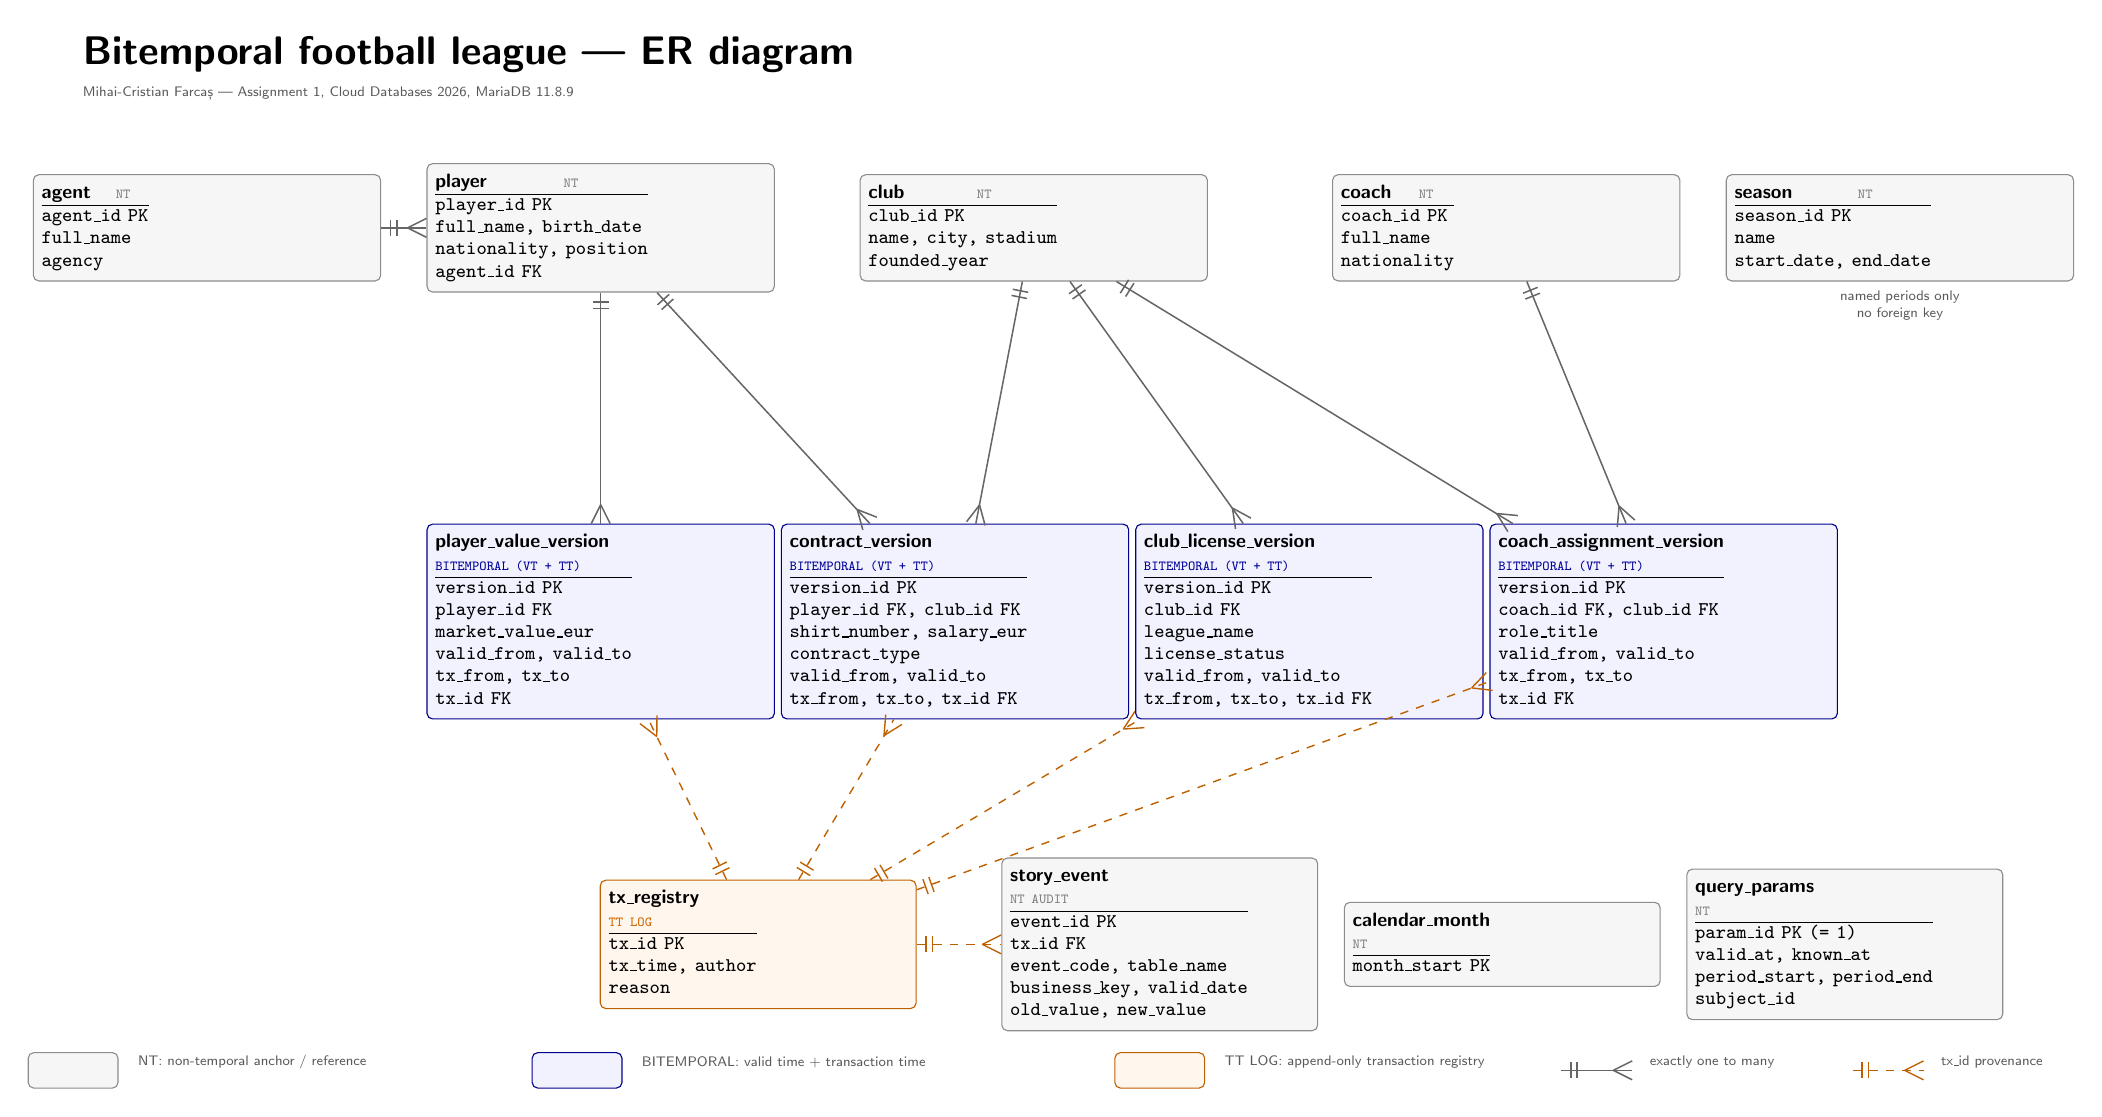
\begin{tikzpicture}

\node[title, anchor=west] at (-0.2,12.4) {Bitemporal football league --- ER diagram};
\node[note, anchor=west] at (-0.2,11.9)
  {Mihai-Cristian Farca\textcommabelow{s} --- Assignment 1, Cloud Databases 2026, MariaDB 11.8.9};

% non-temporal anchors

\node[nt] (agent) at (1.5,10.2) {\begin{tabular}{@{}l@{}}
  \textbf{\sffamily agent} \hfill \textcolor{gray}{\tiny NT}\\
  \hline
  agent\_id PK\\
  full\_name\\
  agency
\end{tabular}};

\node[nt] (player) at (6.5,10.2) {\begin{tabular}{@{}l@{}}
  \textbf{\sffamily player} \hfill \textcolor{gray}{\tiny NT}\\
  \hline
  player\_id PK\\
  full\_name, birth\_date\\
  nationality, position\\
  agent\_id FK
\end{tabular}};

\node[nt] (club) at (12.0,10.2) {\begin{tabular}{@{}l@{}}
  \textbf{\sffamily club} \hfill \textcolor{gray}{\tiny NT}\\
  \hline
  club\_id PK\\
  name, city, stadium\\
  founded\_year
\end{tabular}};

\node[nt] (coach) at (18.0,10.2) {\begin{tabular}{@{}l@{}}
  \textbf{\sffamily coach} \hfill \textcolor{gray}{\tiny NT}\\
  \hline
  coach\_id PK\\
  full\_name\\
  nationality
\end{tabular}};

\node[nt] (season) at (23.0,10.2) {\begin{tabular}{@{}l@{}}
  \textbf{\sffamily season} \hfill \textcolor{gray}{\tiny NT}\\
  \hline
  season\_id PK\\
  name\\
  start\_date, end\_date
\end{tabular}};

% bitemporal version tables

\node[bt] (value) at (6.5,5.2) {\begin{tabular}{@{}l@{}}
  \textbf{\sffamily player\_value\_version}\\
  \textcolor{blue!60!black}{\tiny BITEMPORAL (VT + TT)}\\
  \hline
  version\_id PK\\
  player\_id FK\\
  market\_value\_eur\\
  valid\_from, valid\_to\\
  tx\_from, tx\_to\\
  tx\_id FK
\end{tabular}};

\node[bt] (contract) at (11.0,5.2) {\begin{tabular}{@{}l@{}}
  \textbf{\sffamily contract\_version}\\
  \textcolor{blue!60!black}{\tiny BITEMPORAL (VT + TT)}\\
  \hline
  version\_id PK\\
  player\_id FK, club\_id FK\\
  shirt\_number, salary\_eur\\
  contract\_type\\
  valid\_from, valid\_to\\
  tx\_from, tx\_to, tx\_id FK
\end{tabular}};

\node[bt] (licence) at (15.5,5.2) {\begin{tabular}{@{}l@{}}
  \textbf{\sffamily club\_license\_version}\\
  \textcolor{blue!60!black}{\tiny BITEMPORAL (VT + TT)}\\
  \hline
  version\_id PK\\
  club\_id FK\\
  league\_name\\
  license\_status\\
  valid\_from, valid\_to\\
  tx\_from, tx\_to, tx\_id FK
\end{tabular}};

\node[bt] (assignment) at (20.0,5.2) {\begin{tabular}{@{}l@{}}
  \textbf{\sffamily coach\_assignment\_version}\\
  \textcolor{blue!60!black}{\tiny BITEMPORAL (VT + TT)}\\
  \hline
  version\_id PK\\
  coach\_id FK, club\_id FK\\
  role\_title\\
  valid\_from, valid\_to\\
  tx\_from, tx\_to\\
  tx\_id FK
\end{tabular}};

% registry and helper tables

\node[aud] (tx) at (8.5,1.1) {\begin{tabular}{@{}l@{}}
  \textbf{\sffamily tx\_registry}\\
  \textcolor{orange!80!black}{\tiny TT LOG}\\
  \hline
  tx\_id PK\\
  tx\_time, author\\
  reason
\end{tabular}};

\node[ntsmall] (story) at (13.6,1.1) {\begin{tabular}{@{}l@{}}
  \textbf{\sffamily story\_event}\\
  \textcolor{gray}{\tiny NT AUDIT}\\
  \hline
  event\_id PK\\
  tx\_id FK\\
  event\_code, table\_name\\
  business\_key, valid\_date\\
  old\_value, new\_value
\end{tabular}};

\node[ntsmall] (calendar) at (17.95,1.1) {\begin{tabular}{@{}l@{}}
  \textbf{\sffamily calendar\_month}\\
  \textcolor{gray}{\tiny NT}\\
  \hline
  month\_start PK
\end{tabular}};

\node[ntsmall] (params) at (22.3,1.1) {\begin{tabular}{@{}l@{}}
  \textbf{\sffamily query\_params}\\
  \textcolor{gray}{\tiny NT}\\
  \hline
  param\_id PK (= 1)\\
  valid\_at, known\_at\\
  period\_start, period\_end\\
  subject\_id
\end{tabular}};

% relationships

\connect{agent}{player}
\connect{player}{value}
\connect{player}{contract}
\connect{club}{contract}
\connect{club}{licence}
\connect{coach}{assignment}
\connect{club}{assignment}
\connectd{tx}{contract}
\connectd{tx}{value}
\connectd{tx}{licence}
\connectd{tx}{assignment}
\connectd{tx}{story}

% season has no foreign key
\node[note, anchor=north] at (season.south) {named periods only\\no foreign key};

% legend

\begin{scope}[shift={(-0.2,-0.5)}]
  \node[nt, minimum width=1.0cm, minimum height=0.45cm, text width=1.0cm, inner sep=2pt] (l1) at (0,0) {};
  \node[note, anchor=west] at (0.7,0.1) {NT: non-temporal anchor / reference};
  \node[bt, minimum width=1.0cm, minimum height=0.45cm, text width=1.0cm, inner sep=2pt] (l2) at (6.4,0) {};
  \node[note, anchor=west] at (7.1,0.1) {BITEMPORAL: valid time + transaction time};
  \node[aud, minimum width=1.0cm, minimum height=0.45cm, text width=1.0cm, inner sep=2pt] (l3) at (13.8,0) {};
  \node[note, anchor=west] at (14.5,0.1) {TT LOG: append-only transaction registry};
  \legendrel{18.9}{erd}
  \node[note, anchor=west] at (19.9,0.1) {exactly one to many};
  \legendrel{22.6}{erdd}
  \node[note, anchor=west] at (23.6,0.1) {tx\_id provenance};
\end{scope}

\end{tikzpicture}
\end{document}
